\section{The \textbf{TransP-0} design space}
%\section{The \textbf{TransP-0} integrated design abstraction}
\label{proposed_model}
The \textsc{TransP-0} design framework is intended to support both transportation and power system engineers
during early project phases 
in formulating and evaluating different design options quickly. Therefore, transportation and energy system properties - both static and dynamic - have to be captured sufficiently precise. On the other hand, the design abstraction should omit unnecessary details to enable frequent design iterations. With these requirements in mind we have developed a candidate design abstraction, which is summarized in Figure~\ref{system_design}. The abstraction comprises various transportation and energy subsystem parameters. Note that we focused on using a minimum number of parameters, considering potentially decreased physical accuracy. However, to capture the real-world environment and establish a well-founded terminology, it is important to establish formal definitions.
\begin{figure}[h!]
	\begin{center}
	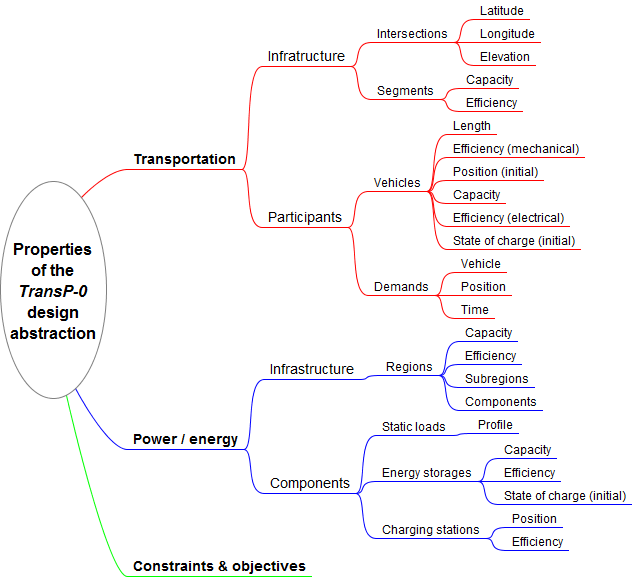
\includegraphics[trim=0 10 0 0, width=0.875\columnwidth]{./gfx/system_design.png}
	\caption{Overview over the \textsc{TransP-0} design space parameters comprising the transportation and the energy subsystem.}
	\label{system_design}
	\end{center}
\end{figure}

Formally, the design space $DS$ of the integrated design abstraction is modeled as a tuple $(TS, ES)$, where
\begin{itemize}
	\item $TS$ represents the \textit{transportation subsystem} and
	\item $ES$ represents the \textit{energy subsystem}.
\end{itemize}
Subsequently we formally describe the design space parameters for the transportation subsystem in Section~\ref{transport} and the energy subsystem in Section~\ref{energy_system}.

\subsection{Transportation subsystem}
\label{transport}

%why is it mesoscopic?
We decided to model the transportation subsystem in a mesoscopic fashion \cite{burghout2005mesoscopic}. In particular, our model includes a representation of the road network and the individual vehicles. The road network is modeled as a directed graph, where nodes represent intersections and edges represent road segments. Hereby, the edge weight defines the number of lanes and the edge direction indicates the intended driving direction.
%Consequently, two edges have to be used to describe bidirectional traffic flows. 
%Here, the vehicles represent ''particles'' that are traveling along the road network. 
Vehicles are assigned to points on the edges of the road network. Hence, vehicles are able to move along edges and switch between edges at intersections. The \textsc{TransP-0} abstraction of the transportation subsystem is illustrated in Figure~\ref{transport_illustration}.

\begin{figure}[h]
	\begin{center}
	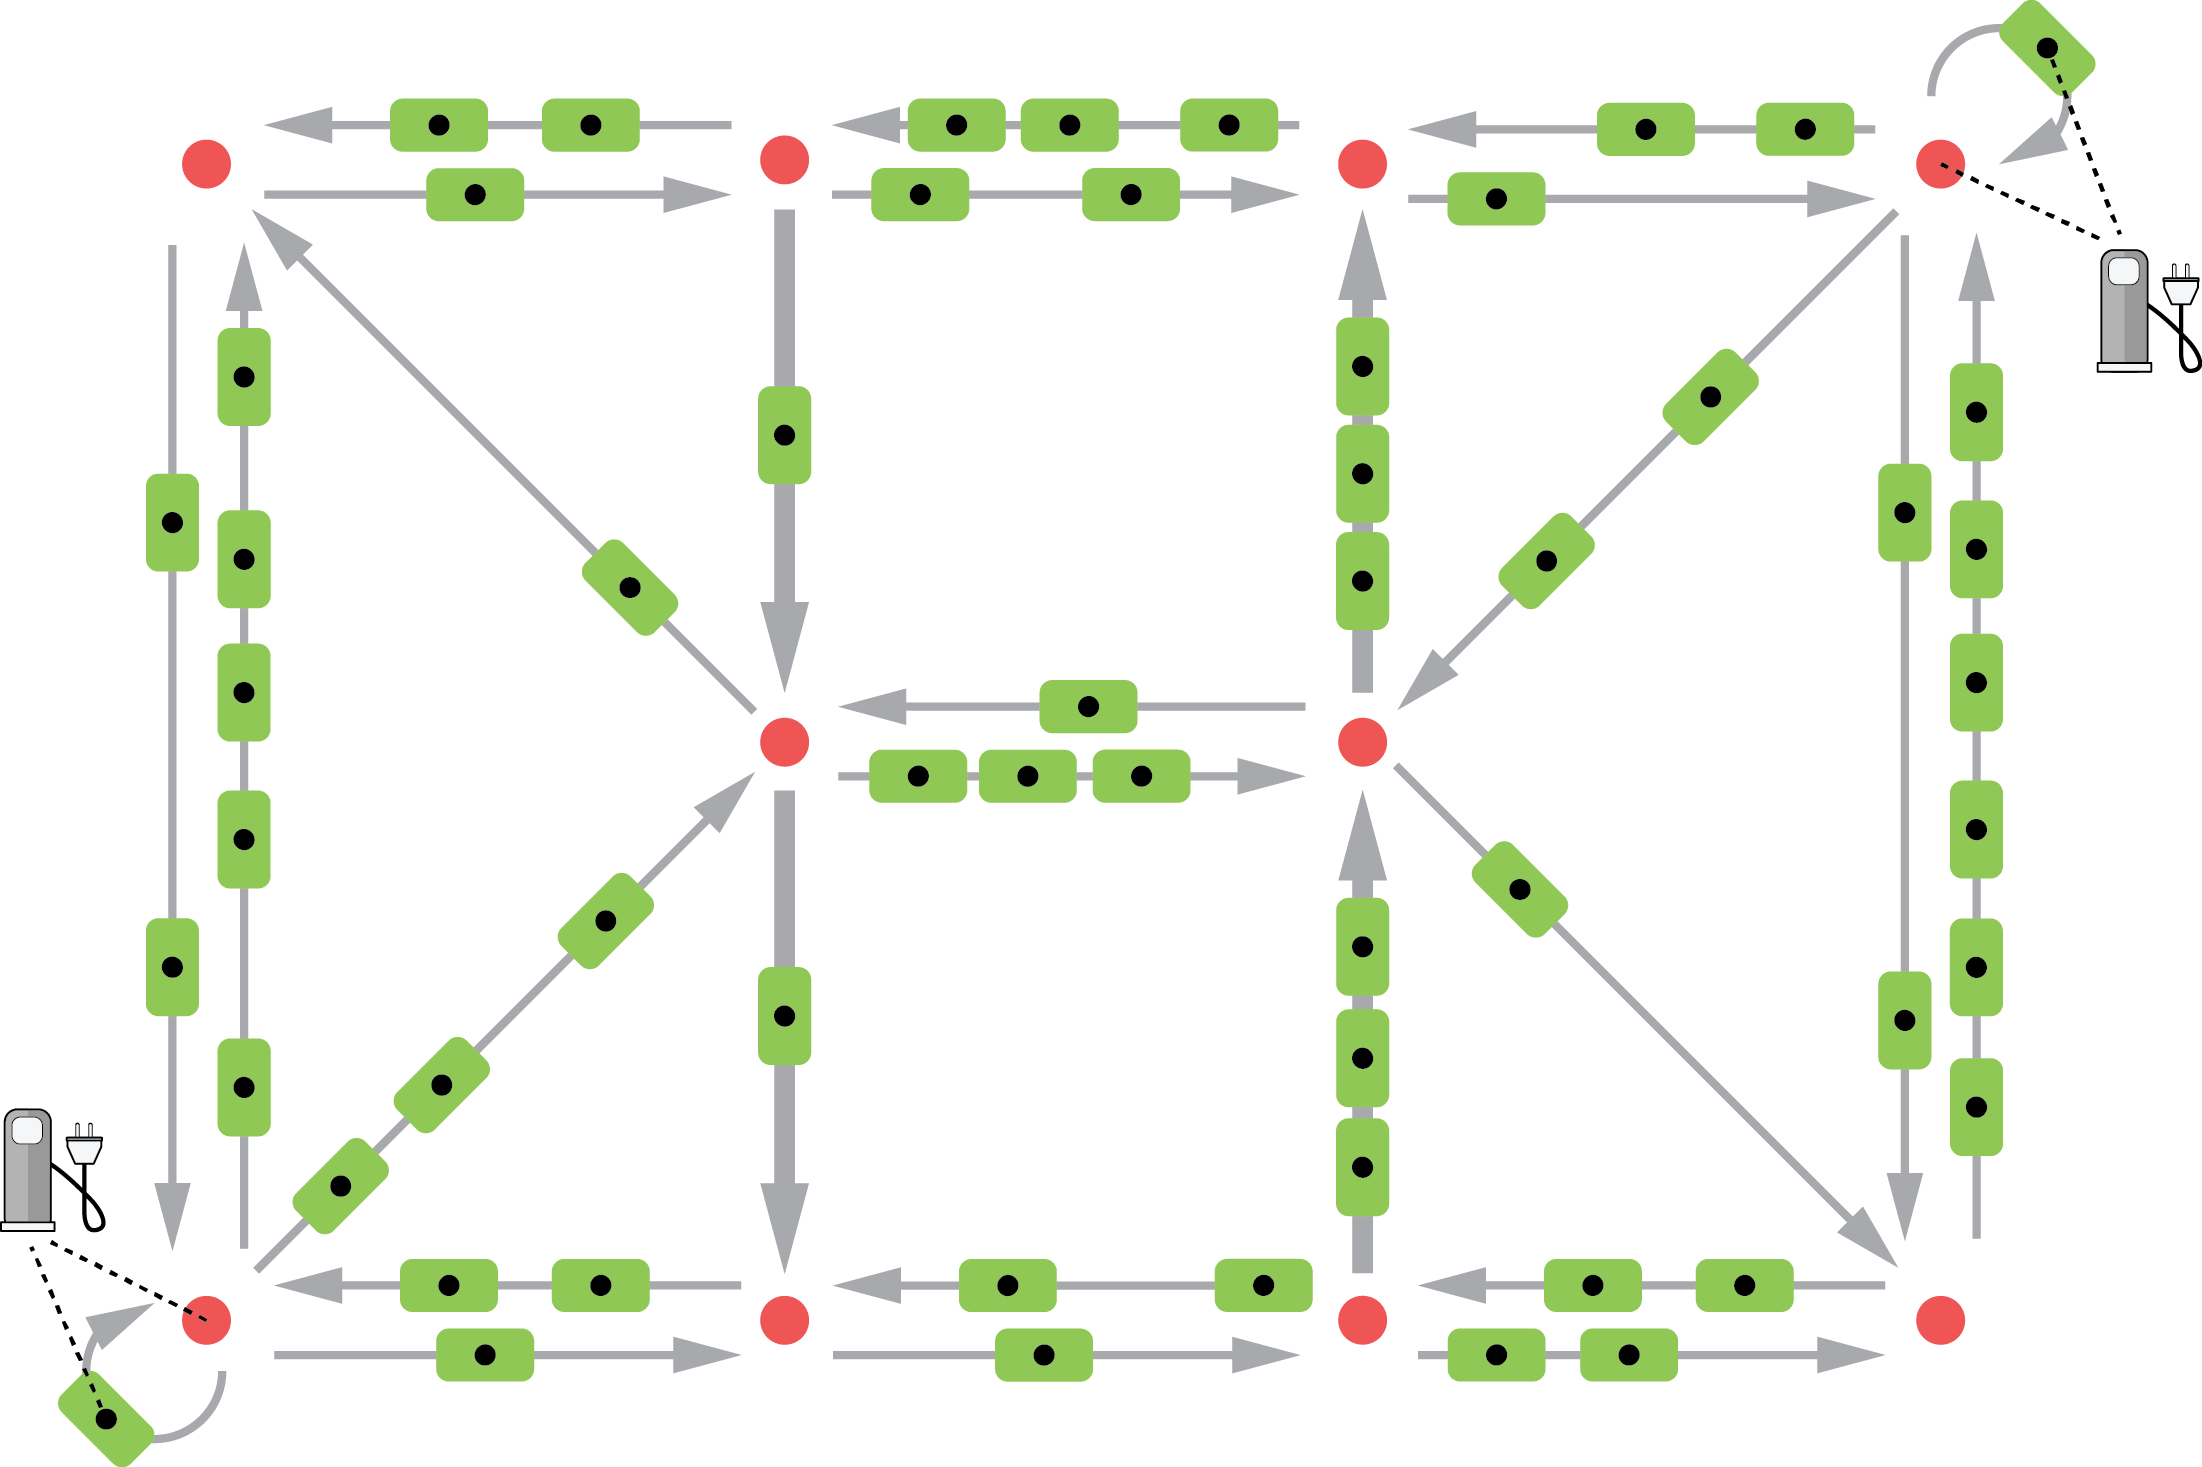
\includegraphics[trim=0 6 0 21, width=.9\columnwidth]{./gfx/transportation_system.png}
	\caption{Representation of the transportation subsystem including an infrastructure (i.e.\ \textit{red} road intersections and \textit{gray} segments) and \textit{green} participants.}
	\label{transport_illustration}
	\end{center}
\end{figure}

Formally, the transportation subsystem $TS$ of the integrated design abstraction is modeled as a tuple $(TI, TP)$, where
\begin{itemize}
	\item $TI$ represents the \textit{transportation infrastructure} and
	\item $TP$ represents the \textit{traffic participants}.
\end{itemize}
Essentially, we distinguish between the static (i.e.\ the infrastructure) and the dynamic (i.e.\ the participants) parts of the transportation subsystem. In the following, we describe the the infrastructure design abstraction in Section~\ref{transport_infrastructure} before explaining the participant design abstraction in Section~\ref{participants}.

\subsubsection{Infrastructure}
\label{transport_infrastructure}

The transportation infrastructure $TI$ is modeled as a tuple $(RI, RS)$, where
\begin{itemize}
	\item $RI$ represents the \textit{road intersections} and
	\item $RS$ represents the \textit{road segments}.
\end{itemize}
Road intersections describe the nodes of the directed graph, while road segments describe the edges instead. Subsequently, we first describe road intersections in Section~\ref{intersections} before explaining road segments in Section~\ref{segments}.

\paragraph{Intersections}
\label{intersections}

%The road intersections $RI$ are modeled as a tuple $(RIL, RIC)$, where
%\begin{itemize}
%	\item $RIL$ represents a finite set of road intersection \textit{labels} and
%	\item $RIC: RIL \rightarrow \mathbb{R}^3$ represents a mapping from road intersection labels to geometric \textit{coordinates}.
%\end{itemize}

The road intersections $ri \in RI$ are modeled as a one-tuple $(ri_c)$, where
\begin{itemize}
	\item $ri_c\in \mathbb{R}^3$ represents their geometric \textit{coordinates}.
\end{itemize}

%Note that typically the coordinates are expressed in terms of latitude, longitude, and elevation (see Figure~\ref{system_design}). However, for simplicity in this work we use Cartesian coordinates instead.

\paragraph{Segments}
\label{segments}

	Instead, the road segments $rs \in RS$ are modeled as a four-tuple $(rs_s, rs_t, rs_c, rs_e)$, where
	\begin{itemize}
		\item $rs_{s/t} \in RI$ represent their \textit{source} and \textit{target} road intersections,
		\item $rs_c \in \mathbb{N}$ represents their \textit{capacities} (i.e.\ the number of lanes), and
		\item $rs_e \in \mathbb{R}^+$ represents their \textit{efficiency} (i.e.\ a friction coefficient).
	\end{itemize}
	Note that the previous parameters completely determine our road segment model. Consequently, we abstract from a variety of parameters typically considered in microscopic models such as continuous elevation profiles. However, our model supports arbitrary discretization as distance between intersections and the length of edges can be chosen arbitrarily.


%\textcolor{red}{
%	Instead, the road segments $RS$ are modeled as a five-tuple $(RSL, RSS, RST, RSC, RSE)$, where
%	\begin{itemize}
%		\item $RSL$ represents a finite set of road segment \textit{labels},
%		\item $RSS/RST: RSL \rightarrow RIL$ represent mappings from road segment labels to their respective \textit{source} and \textit{target} road intersection labels and accounts for self-edges,
%		\item $RSC: RSL \rightarrow \mathbb{N}$ represents a mapping from road segment labels to their \textit{capacities} (i.e.\ the number of lanes of the road segment), and
%		\item $RSE: RSL \rightarrow \mathbb{R}^+$ represents a mapping from road segment labels to their \textit{efficiency} (i.e.\ a friction coefficient of the road segment).
%	\end{itemize}
%	Note that the previous parameters completely determine our road segment model. Consequently, we abstract from a variety of parameters typically considered in microscopic models such as continuous elevation profiles. However, our model supports arbitrary discretization as distance between intersections and the length of edges can be chosen arbitrarily.
%	%quelle
%}
\textcolor{red}{
Furthermore, we derive the road segment distance $RSD: RS \rightarrow \mathbb{R}_0^+$ as a mapping from road segments to distances using the Euclidean metric $E: \mathbb{R}^3 \times \mathbb{R}^3 \rightarrow \mathbb{R}_0^+$ such that
\[
	RSD(rs) = E(RIC(rs_s), RIC(rs_t)) \textrm{.}
\]
Finally, we define road segment positions $RSP \subseteq RS \times \mathbb{R}_0^+$ as tuples of road segments and traveled distances
\[
	RSP = \{(rs, d) \in RS \times \mathbb{R}_0^+ \mid d \leq RSD(rs)\} \textrm{.}
\]
We use the road segment positions $RSP$ to locate traffic participants (i.e.\ vehicles) on the transportation infrastructure as explained in the following section. 
}
%Note that the world coordinates can be obtained by a respective coordinate transformation.

\subsubsection{Participants}
\label{participants}

The traffic participants $TP$ are modeled as a tuple $(V, D)$, where
\begin{itemize}
	\item $V$ represents the \textit{vehicles} and
	\item $D$ represents the \textit{demands}.
\end{itemize}
Consequently, we - again - distinguish between static (i.e.\ the vehicles) and dynamic (i.e.\ the demands) properties of the model. In the following, we first describe the vehicle design abstraction in Section~\ref{vehicles} before explaining the demand design abstraction in Section~\ref{demands}.

\paragraph{Vehicles}
\label{vehicles}

%The vehicles $V$ are modeled as a seven-tuple $(VL, VS, VME, VP_0, VC, VEE, VSOC_0)$, where
%\begin{itemize}
%	\item $VL$ represents a finite set of vehicle \textit{labels},
%	\item $VS: VL \rightarrow \mathbb{R}^+$ represents a mapping from vehicle labels to their \textit{size} (i.e.\ the length of the vehicle in road segment direction),
%	\item $VME: VL \rightarrow \mathbb{R}^+$ represents a mapping from vehicle labels to their \textit{mechanical efficiency} (i.e. the conversion coefficient between employed energy and driven distance similar to \cite{gao2007modeling}),
%	%(i.e.\ a constant ratio for conversion between electrical and mechanical energy),
%	\item $VP_0: VL \rightarrow RSP$ represents a mapping from vehicle labels to their initial road segment \textit{positions} (see Section~\ref{segments}),
%	\item $VC: VL \rightarrow \mathbb{R}^+$ represents a mapping from vehicle labels to their battery \textit{capacities} (i.e.\ the maximum amount of energy that can be stored by the vehicle),
%	\item $VEE: VL \rightarrow \mathbb{R}^+$ represents a mapping from vehicle labels to their \textit{electrical efficiency} (i.e. the conversion coefficient between employed and stored energy),
%	%(i.e.\ a constant ratio for conversion between electrical and stored energy), and
%	\item $VSOC_0: VL \rightarrow \mathbb{R}^+$ represents a mapping from vehicle labels to their initial \textit{state of charge} (i.e.\ the amount of energy stored by the vehicle initially) such that
%	\[
%		\forall vl \in VL : VSOC_0(vl) \leq VC(vl) \textrm{.}
%	\]
%\end{itemize}
%Note that we again abstract from many parameters which can be considered in microscopic models \cite{gao2007modeling} such as vehicle weight or exact vehicle geometry. In particular, we approximate mechanical and electrical efficiencies with constants only.

The vehicles $v \in V$ are modeled as a six-tuple $(v_s, v_{me}, v_p^0, v_c, v_{ee}, v_{soc}^0)$, where
\begin{itemize}
	\item $v_s \in \mathbb{R}^+$ represents their \textit{size} (i.e.\ the length of the vehicle in road segment direction),
	\item $v_{me} \in \mathbb{R}^+$ represents their \textit{mechanical efficiency} (i.e. the conversion coefficient between employed energy and driven distance similar to \cite{gao2007modeling}),
	%(i.e.\ a constant ratio for conversion between electrical and mechanical energy),
	\item $v_p^0 \in RSP$ represents their initial road segment \textit{positions} (see Section~\ref{segments}),
	\item $v_c \in \mathbb{R}^+$ represents their battery \textit{capacities} (i.e.\ the maximum amount of energy that can be stored by the vehicle),
	\item $v_{ee} \in \mathbb{R}^+$ represents their \textit{electrical efficiency} (i.e. the conversion coefficient between employed and stored energy),
	%(i.e.\ a constant ratio for conversion between electrical and stored energy), and
	\item $v_{soc}^0 \in \mathbb{R}^+$ represents their initial \textit{state of charge} (i.e.\ the amount of energy stored by the vehicle initially) such that
	\[
	\forall v \in V : v_{soc}^0 \leq v_c \textrm{.}
	\]
\end{itemize}
Note that we again abstract from many parameters which can be considered in microscopic models \cite{gao2007modeling} such as vehicle weight or exact vehicle geometry. In particular, we approximate mechanical and electrical efficiencies with constants only.

\paragraph{Demands}
\label{demands}

Finally, the demands $d \in D$ are modeled as a three-tuple $(d_v, d_p, d_t)$, where
\begin{itemize}
	\item \textcolor{red}{$d_v \in V$ represents the demand of a vehicle (i.e.\ the concerned vehicle),}
	\item $d_p \in RSP$ represents the demand at road segments \textit{positions} (i.e.\ where the concerned vehicle is expected to be), and
	\item $d_t \in \mathbb{N}^+$ represents the demand at \textit{time} points (i.e.\ when the concerned vehicle is expected to be there).
\end{itemize}

%Finally, the demands $D$ are modeled as a four-tuple $(DL, DV, DP, DT)$, where
%\begin{itemize}
%	\item $DL$ represents a finite set of demand \textit{labels},
%	\item $DV: DL \rightarrow VL$ represents a mapping from demand labels to \textit{vehicle} labels (i.e.\ the concerned vehicle),
%	\item $DP: DL \rightarrow RSP$ represents a mapping from demand labels to road segment \textit{positions} (i.e.\ where the concerned vehicle is expected to be), and
%	\item $DT: DL \rightarrow \mathbb{N}^+$ represents a mapping from demand labels to \textit{time} points (i.e.\ when the concerned vehicle is expected to be there).
%\end{itemize}

Note that our abstraction is based on discrete time (see Section~\ref{dynamics}). However, we do not prescribe the time step resolution. For long travel distances and durations more coarse resolutions can be used, while for shorter distances and durations more fine-grained resolutions are typically needed.

\subsection{Power / energy subsystem}
\label{energy_system}

Similar to the transportation subsystem (see Section~\ref{transport}), we decided to model the energy subsystem in a mesoscopic fashion~\cite{Hackenberg2012}. Note that microscopic models represent the individual power lines and their physical characteristics~\cite{Dommel1968}, while macroscopic models aggregate the entire energy subsystem into a single marketplace without power line characteristics~\cite{Castronuovo2004}. Our mesoscopic model takes an intermediate approach, where only selected characteristics of the network topology are represented. In particular, we limit our representation to subnetworks of equal voltage level (i.e.\ the network \textit{regions}) and their hierarchical connectivity through transformers. Consequently, balances can be computed also for single regions rather than the entire electricity market. The \textsc{TransP-0} abstraction of the energy subsystem is illustrated in Figure~\ref{energy_illustration}.

\begin{figure}[h]
	\begin{center}
	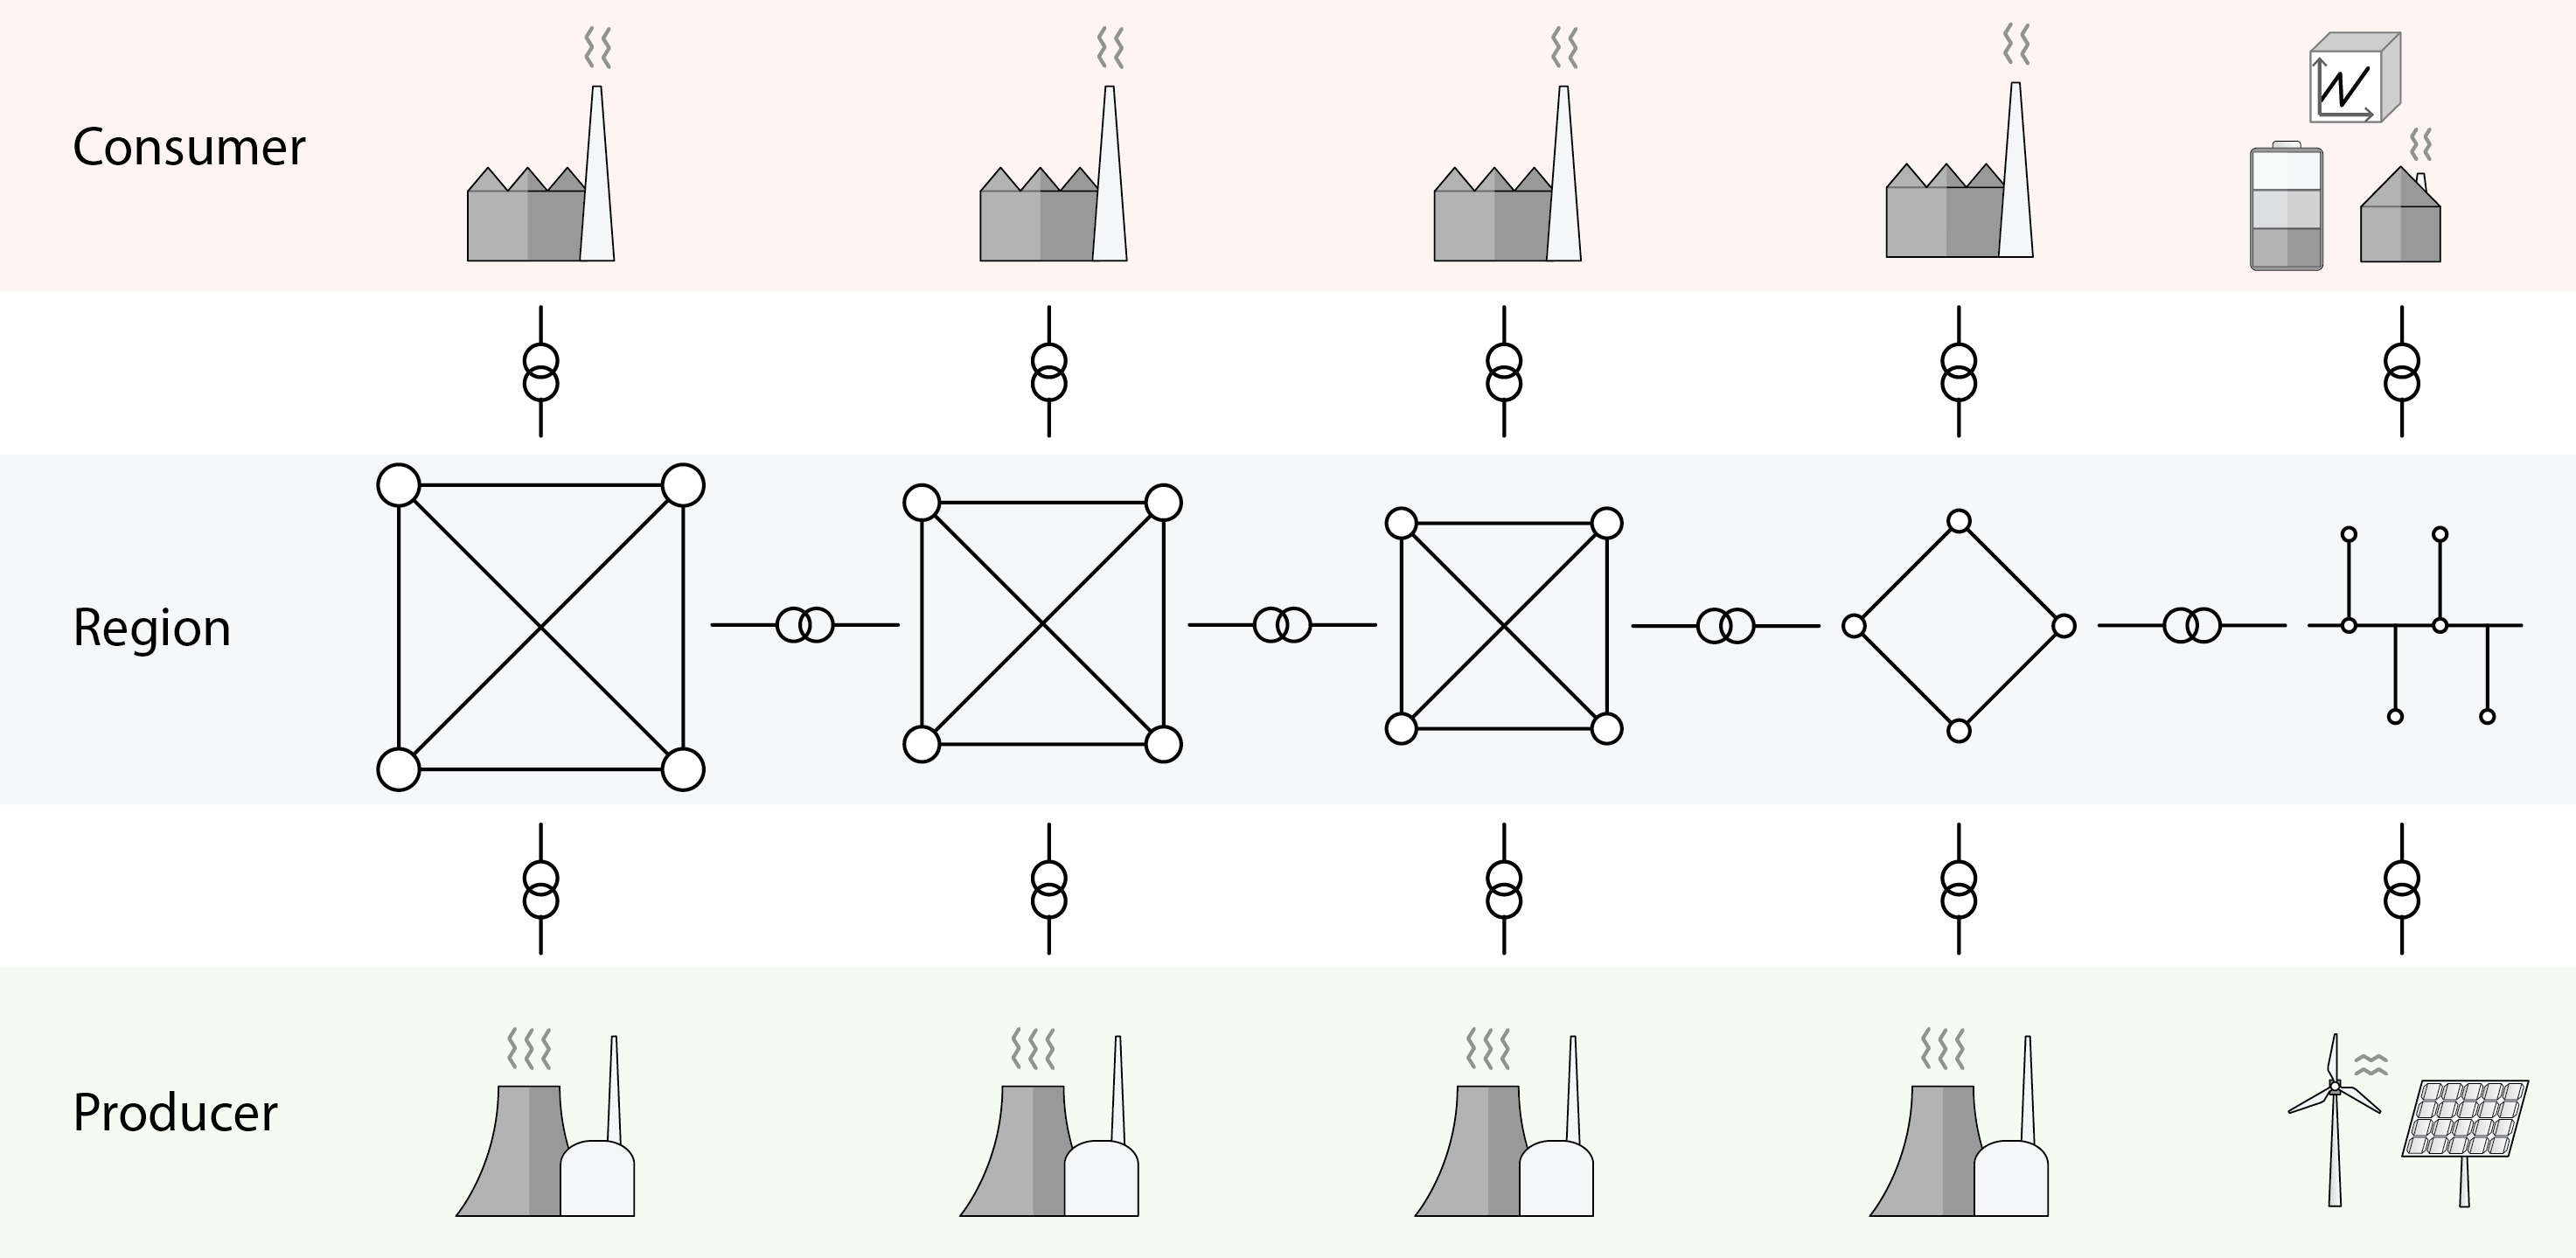
\includegraphics[trim=0 10 0 15, width=0.95\columnwidth]{./gfx/energy_system.png}
	\caption{Illustration of a energy subsystem design including an infrastructure (i.e.\ regions) and components (i.e.\ producers and consumers).}
	\label{energy_illustration}
	\end{center}
\end{figure}

Formally, the energy subsystem $ES$ of the integrated design abstraction is modeled as a tuple $(EI, EC)$, where
\begin{itemize}
	\item $EI$ represents the \textit{energy infrastructure} and
	\item $EC$ represents \textit{energy components}.
\end{itemize}
Hence, we separate network characteristics and network usage. Subsequently, we first explain the infrastructure in Section~\ref{regions} before describing the components in Section~\ref{components}.

\subsubsection{Infrastructure}
\label{energy_infrastructure}

The energy infrastructure $EI$ is modeled as a one-tuple $(R)$, where
\begin{itemize}
	\item $R$ represents the \textit{regions} of the energy infrastructure, which are determined by the voltage levels and transformers of the network.
\end{itemize}
Note that we selected a region model~\cite{Hackenberg2012} over a power flow model~\cite{Dommel1968} to reduce modeling effort and increase computational efficiency. Hence, we think it is important to enable rapid formulation and evaluation. In the following, we describe the regions in Section~\ref{regions}.

\paragraph{Regions}
\label{regions}

The network regions $r \in R$ are modeled as a three-tuple $(r_c, r_e, r_p)$, where
\begin{itemize}
	\item $r_c \in \mathbb{R}^+$ represents their \textit{capacities} (i.e.\ the maximum amount of energy that can flow through each region in a predefined time interval),
	\item $r_e \in \mathbb{R}^+$ represents their \textit{efficiencies} (i.e.\ a constant factor determining the energy that is lost while flowing through that region), and
	\textcolor{red}{
	\item $r_p \in R \cup \{\bot\}$ represents their \textit{parent} regions (i.e.\ the superordinate voltage level or the start symbol $\bot$ for the root level).
}
\end{itemize}
Note that our region model represents the energy system as a tree structure. The nodes of the tree represent \textit{subnetworks} with distinct voltage levels. The edges of the tree represent \textit{transformers} connecting the subnetworks instead. The region model can be derived from existing network topologies easily.

\subsubsection{Components}
\label{components}

Instead, the energy components $EC$ are modeled as a three-tuple $(SL, ES, CS)$, where
\begin{itemize}
	\item $SL$ represents the \textit{static loads},
	\item $ES$ represents the \textit{energy storages}, and
	\item $CS$ represents the \textit{charging stations}.
\end{itemize}
In the following, we first explain the static load design abstraction in Section~\ref{static_loads}, before describing the energy storage design abstraction in Section~\ref{energy_storages} and presenting the charging station design abstraction in Section~\ref{charging_stations}. Note that currently we do not include energy producers such as generators as well as smart consumers. However, these components are subject for our future work.

\paragraph{Static loads}
\label{static_loads}

The static loads $sl \in SL$ are modeled as a two-tuple $(sl_p, sl_r)$, where
\begin{itemize}
	\item \textcolor{red}{$sl_p \in (\mathbb{N} \rightarrow \mathbb{R})$ represents their static load \textit{profiles} (i.e.\ a predefined production and consumption curve), and}
	\item $sl_r \in R$ represents their parent \textit{regions} (i.e.\ the region where the static load is attached).
\end{itemize}
Note that static load profiles associate a numeric load to each discrete time step. Hereby positive loads represent energy production and negative loads represent energy consumption. Consequently, static loads can be used to model everything from home appliances over solar panels to conventional power generators. In particular, we assume such loads to be uncontrollable from the perspective of the engineers.

\paragraph{Energy storages}
\label{energy_storages}

Then, the energy storages $es \in ES$ are modeled as a four-tuple $(es_c, es_e, es_s^0, es_r)$, where
\begin{itemize}
	\item $es_c \in \mathbb{R}^+$ represents their \textit{capacities} (i.e.\ the maximum amount of energy that can be stored),
	\item $es_e \in \mathbb{R}^+$ represents their \textit{efficiencies} (i.e. the conversion coefficient between  and stored energy), and
	\item $es_s^0 \in \mathbb{R}_0^+$ represents their initial \textit{state of charges} (i.e.\ the amount of energy stored initially) such that
	\[
		 \textcolor{red}{ es_s^0 \leq es_c \textrm{, and} }
	\]
	\item $es_r \in R$ represents their parent \textit{regions} (i.e.\ the region where the energy storage is attached).
\end{itemize}
Note that the energy storage model is analogous to the electric vehicle model described in Section~\ref{vehicles}. However, electric vehicles additionally define mechanical parameters, while energy storages are attached to regions statically. Furthermore, we currently target small batteries rather than large storage facilities. Note that the latter might require additional parameters. 
%Larger facilities require additional parameters~\cite{?}.

\paragraph{Charging stations}
\label{charging_stations}

Finally, the charging stations $cs \in CS$ are modeled as a three-tuple $(cs_p, cs_e, cs_r)$, where
\begin{itemize}
	\item $cs_e \in \mathbb{R}^+$ represents their \textit{efficiencies} (i.e.\ a constant loss factor for respective energy flows), and
	\item $cs_p \in RS$ represents their \textit{positions}, i.e.\ road segments with zero road segment distance
	\[
		\textcolor{red}{ RSD(cs_p) = 0 \textrm{, and} }
	\]
	\item $cs_r \in R$ represents their parent \textit{regions} (i.e.\ the region where the charging station is attached).
\end{itemize}
Note that the charging station position $cs_p$ and the charging station parent region $cs_r$ define the static connections between the transportation subsystem and the energy subsystem. Consequently, vehicles (see Section~\ref{vehicles}) are able to interact with arbitrary regions (see Section~\ref{regions}) of the energy subsystem infrastructure at predefined zero-length road segments (see Section~\ref{segments}).
